
% Inbuilt themes in beamer
\documentclass{beamer}
\usepackage{graphicx}
% Theme choice:
\usetheme{CambridgeUS}

% Title page details: 
\title{Elements of Microeconomics: \\
       Discussion Section 4} 
\author{John Green}
\date{September 1, 2023}


\begin{document}

% Title page
\begin{frame}
    \titlepage 
\end{frame}

% Outline frame
\begin{frame}{Outline}
    This week will cover chapters 1 and 2 of the Mankiw textbook:
    \begin{enumerate}
        \item Ten principles of economics
        \item Thinking like an economist
    \end{enumerate}

    \medskip

    Essentially just a gentle introduction: 
    \begin{itemize}
        \item What is economics?
        \item What do economists do?
        \item How do economists think?
    \end{itemize}
\end{frame}

\begin{frame}{Main point}
    \centering
    Main takeaway from this week:

    \vspace{12pt}

    \Large \textit{A little bit of intuition goes a long way.}

    \normalsize There is usually a nice everyday analogy for questions in microeconomics. 
\end{frame}

\section{Chapter 1: Ten Principles}

% How people make decisions
\begin{frame}{How people make decisions}
    \begin{block}{1. People face trade-offs.}
        There are finite and scarce resources.
    \end{block}

    \begin{block}{2. The cost of something is what you give up to get it.}
        Everything is opportunity cost!
    \end{block}

    \begin{block}{3. Rational people think at the margin}
        What will a small change in X do to Y?
    \end{block}

    \begin{block}{4. People respond to incentives}
        How can we change behavior?
    \end{block}
\end{frame} 

% How people interact
\begin{frame}{How people make decisions}
    This is the bread and butter of microeconomics!
    
    \medskip

    \begin{block}{5. Trade can make everyone better off.}
        Everyone can do what they do best.
    \end{block}

    \begin{block}{6. Markets are usually a good way to organize economic activity.}
        Markets solve the information problem.
    \end{block}

    \begin{block}{7. Governments can improve market outcomes.}
        What happens when individuals do not internalize their costs?
    \end{block}
\end{frame} 

% Economy as a whole
\begin{frame}{How the economy as a whole works}
    Microeconomics aggregates up to macroeconomics.

    \medskip

    \begin{block}{8. A country's standard of living depends on its ability to produce goods and services.}
        Why do we see such large differences between countries?
    \end{block}

    \begin{block}{9. Prices rise when the government prints too much money.}
        Too much money chasing too few goods is one cause of inflation.
    \end{block}

    \begin{block}{10. Short-run trade-off between inflation and unemployment.}
        The ``Phillips Curve."
    \end{block}
    \section{Lists in Beamer}
\end{frame} 

\begin{frame}{Trade-offs}
    You are trying to decide whether to go on a beach trip during your first spring break. What costs do you need to consider? 
\end{frame}

\begin{frame}{Trade-offs}
    You are trying to decide whether to go on a beach trip during your first spring break. What costs do you need to consider? 
    \begin{enumerate}
        \item Dollar cost of the vacation: transportation, food, renting a house \dots
        \item Money you could make if you worked your part-time job instead
        \item Studying you could get done: preparation for finals, work on semester projects, etc.
    \end{enumerate}
\end{frame}

\section{Chapter 2: Thinking like an economist}

\begin{frame}{The economist as scientist}
    Provocative! 

    \medskip

    How are economists like scientists? 
    How are economists not like scientists?

    \medskip

    \begin{block}{“Imagine how much harder physics would be if electrons had feelings.”}
        - Richard Feynman, theoretical physicist
    \end{block}

    \medskip

    Economists work with models, which rest on assumptions. Let's look at a few.
\end{frame}

\begin{frame}
    \frametitle{Circular flow}
    \centering
    \includegraphics[width = 0.7\textwidth,keepaspectratio]{model1.png}
\end{frame}

\begin{frame}
    \frametitle{Production possibility frontier}
    \centering
    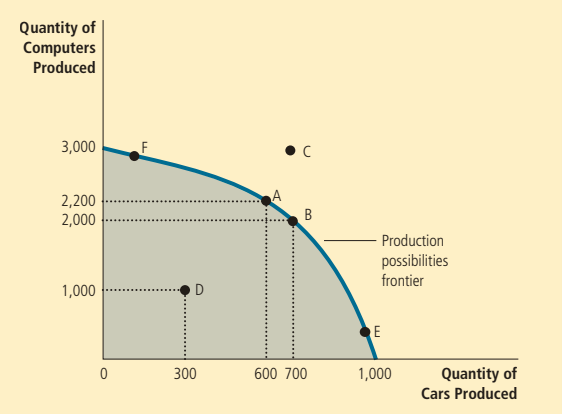
\includegraphics[width = 0.8\textwidth,keepaspectratio]{model2.png}
\end{frame}

\begin{frame}{PPF of a firm}
    Let's start an Italian restaurant that makes pizzas and sandwiches.
    \begin{enumerate}
        \item What will our production possibility frontier look like?
        \item Why will it take the shape that it has?
        \item How can we read the opportunity cost?
        \item Why might the shape change over time?
    \end{enumerate}
\end{frame}

\begin{frame}{CPF of an individual}
    Now suppose we are \textit{going} to the Italian restaurant with a group of friends, and we want to decide what to order. Pizzas are \$10, sandwiches are \$5, and we have \$100 to spend.
    \begin{enumerate}
        \item What will our consumption possibility frontier look like?
        \item What is the opportunity cost of a pizza? Does it matter where on the CPF we are?
        \item What will happen to the CPF if we have \$200 to spend?
        \item What will happen to the CPF if the price of sandwiches increases to \$10?
    \end{enumerate}
\end{frame}

\begin{frame}{Circular-flow diagram of the Italian restaurant economy}
    Suppose the entire economy consists of Italian restaurants: during half of the week we work in one, and during the other half we buy food from them.

    \medskip

    \begin{itemize}
        \item What does the circular-flow diagram look like?
        \item What is missing from our model?
    \end{itemize}

\end{frame}

\begin{frame}
    \frametitle{Economists, economics, and economic reality}    
    Economists are often asked to guide economic policy.
    \begin{itemize}
        \item What are positive and normative statements?
        \item Why might two economists make different suggestions?
        \item Why might politicians ignore economists' suggestions?
    \end{itemize}
\end{frame}

\end{document}